%%%%%%%%%%%%%%%%%%%%%%%%%%%%%%%%%%%%%%%%%%%%%%
%                insertmeeting
% 1) Title (something creative & funny?)
% 2) Date (MM/DD/YYYY)
% 3) Location (ex. Hagerty High School)
% 4) People/Committees Present 
% 5) Picture 
% 6) Start Time & Stop Time (ex. 12:30AM to 4:30PM)
%%%%%%%%%%%%%%%%%%%%%%%%%%%%%%%%%%%%%%%%%%%%%%
\insertmeeting 
	{Let's Get Digital} 
	{09/23/21}
	{Hagerty High School}
	{Austin English, Ryan Nelson}
	{Images/RobotPics/robot.jpg}
	{2:30 - 4:30}
	
\subsection*{Programming}
\noindent\hfil\rule{\textwidth}{.4pt}\hfil
\subsubsection*{Goals}
\begin{itemize}
    \item Set up Android studio
    \item set up TRC code   
    \item Set up a new Github repository for this years code
    \item Help all new programming team members obtain a github account 
\end{itemize} 

\noindent\hfil\rule{\textwidth}{.4pt}\hfil

\subsubsection*{Accomplishments}
Today, we worked on setting up a 4717 github repository so we can wirelessly communicate between different computers relatively seamlessly. The repository has different folders for CAD and Programming, among others. Each subset has different permissions as to who can access it to prevent accidental changes to our CAD or program. First, we had all the new members create new accounts in GitHub, as shown in Figure \ref{fig:pic1}. Everyone contributes to the repository, as shown in Figure \ref{fig:pic2}. In order to communicate these files from one person to another, knowing how to pull and push files will be necessary, as shown in Figures \ref{fig:pic3} and \ref{fig:pic4}. 
 
We accomplished our goals of setting up Android studio and the TRC code.
 

\begin{figure}[ht]
\centering
\begin{minipage}[b]{.50\textwidth}
  \centering
  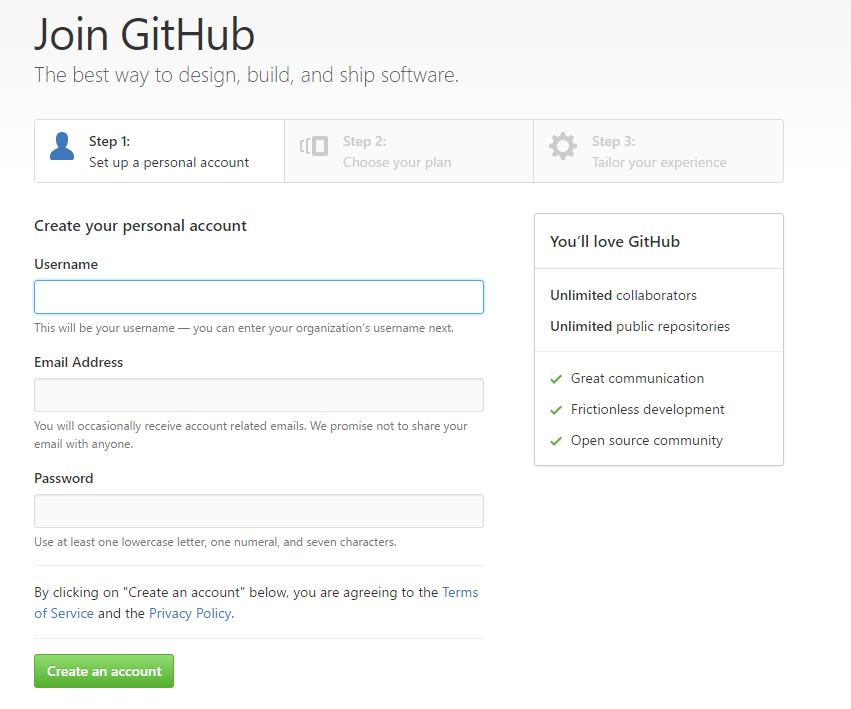
\includegraphics[width=0.5\textwidth]{Meetings/September/09-23-21/githubnewacc.png}
  \caption{New Account in Github}
  \label{fig:pic1}
\end{minipage}%
\hfill%
\begin{minipage}[b]{.50\textwidth}
  \centering
  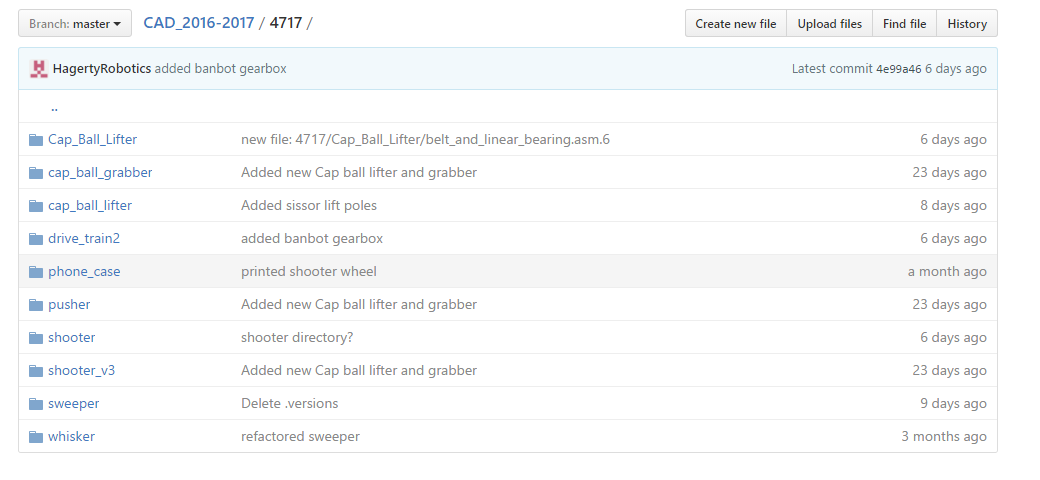
\includegraphics[width=0.8\textwidth]{Meetings/September/09-23-21/githubrepository.png}
  \caption{Screenshot of GitHub Repository}
  \label{fig:pic2}
\end{minipage}
\end{figure}




\begin{figure}
\centering
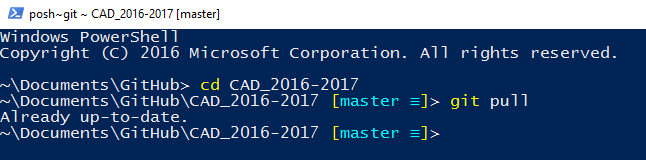
\includegraphics[width=0.85\textwidth, angle=0]{Meetings/September/09-23-21/gitshellpull.png}
\caption{GitShell Pull Files}
\label{fig:pic3}
\end{figure}


\begin{figure}
\centering
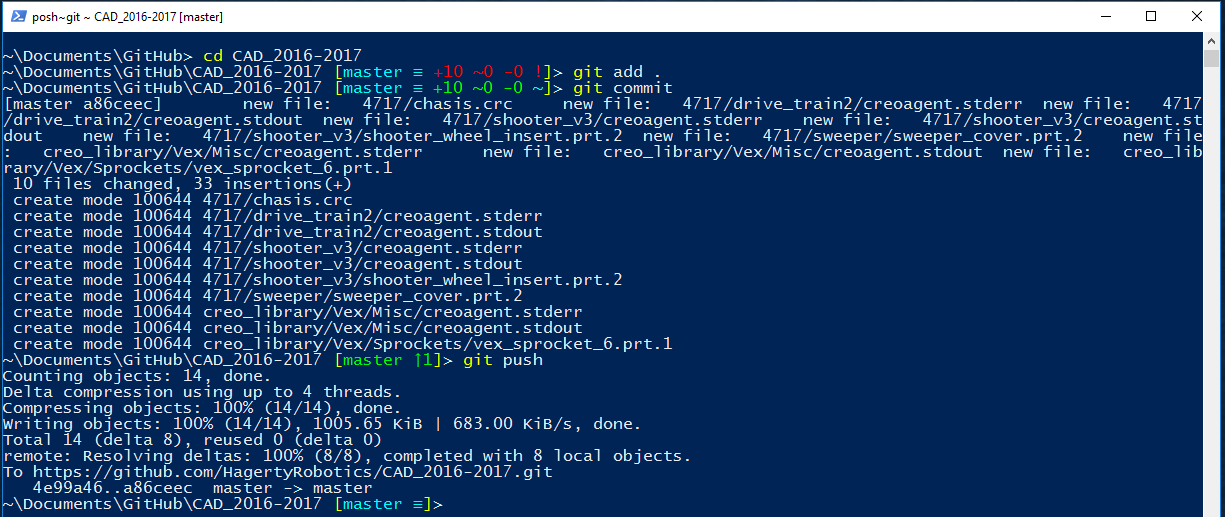
\includegraphics[width=0.85\textwidth, angle=0]{Meetings/September/09-23-21/gitshellpush.png}
\caption{GitShell Push Files}
\label{fig:pic4}
\end{figure}







